\documentclass{article}      % Specifies the document class
%\documentclass[letterpaper,12pt]{article}      % Specifies the document class
%\usepackage[margin=1in]{geometry}              % Set 1-inch margins
\usepackage{caption}
\usepackage[final]{graphicx}
\usepackage{amsmath}
\usepackage{placeins}
\usepackage{float}           % Add float package for [H] option
\title{Case Study 2: Diabetes Dataset - Prediction and Interpretation of Hospital Readmission For Diabetic Patients}  % Declares the document's title.
\author{Kristin Henderson}   % Declares the author's name.
\date{May 27, 2025}          % Deleting this command produces today's date.

\newcommand{\ip}[2]{(#1, #2)}
                             % Defines \ip{arg1}{arg2} to mean
                             % (arg1, arg2).
                             
\begin{document}             % End of preamble and beginning of text.

\maketitle                   % Produces the title.

\section{Introduction}       % Produces section heading.  Lower-level
                             % sections are begun with similar
                             % \subsection and \subsubsection commands.

This study aims to predict hospital readmission into one of three categories: within 30 days, after 30 days, or no readmission, and to identify the variables most associated with readmission risk. This is important because high readmission rates can lead to worse patient outcomes, higher healthcare costs, and increased strain on hospital resources. The dataset used in the analysis is a University of California at Irvine Machine Learning Repository dataset, which contains 101,766 hospital encounters of inpatients diagnosed with diabetes who had hospital stays of 1-14 days, collected from 130 U.S. hospitals between 1999 and 2008. 

\section{Data}
The dataset contains a total of 49 features, both numerical and categorical, plus the multi-class categorical target variable, \texttt{readmitted}. Table 1 contains the features in the dataset grouped roughly by category. The medication features are listed only by broader class. 

\begin{table}[h!]
    \captionof{table}{Features by Broad Category in the Diabetes Dataset} 
    \centering
    \begin{tabular}{|l|p{8cm}|}
    \hline
    \textbf{Broad Category} & \textbf{Features (or Drug Class)} \\ \hline \hline
    ID Variables & encounter\_id, patient\_nbr \\ \hline
    Demographic Variables & race, gender, age, weight \\ \hline
    Admission and Discharge Details & admission\_type\_id, admission\_source\_id, discharge\_disposition\_id \\ \hline
    Administrative Information & time\_in\_hospital, payer\_code, medical\_specialty \\ \hline
    Medical Diagnostics and Treatments & num\_lab\_procedures, num\_procedures, num\_medications, diag\_1, diag\_2, diag\_3, number\_diagnosis \\ \hline
    Previous Hospitalization & num\_outpatient, num\_emergency, num\_inpatient\\ \hline
    Lab Results & max\_glu\_serum, A1Cresult \\ \hline
    Medications & Biguanides, Meglitinides, Sulfonylureas (1st and 2nd generation), Thiazolidinediones, Alpha-Glucosidase Inhibitors, DPP-4 Inhibitors, Insulin, Drug Combinations, Non-Diabetes Medications \\ \hline
    Medication Outcome Variables & change, diabetesMed \\ \hline
    Target & readmitted \\ \hline
    \end{tabular}
    \label{table:features_by_category}
\end{table}

\FloatBarrier
Table 2 contains the medication features grouped by drug class. 

\begin{table}[h!]
    \captionof{table}{Medication Features by Drug Class} 
    \centering
    \begin{tabular}{|l|p{9cm}|}
    \hline
    \textbf{Drug Class} & \textbf{Medications} \\ \hline \hline
    Biguanides & metformin \\ \hline
    Meglitinides & repaglinide, nateglinide \\ \hline
    Sulfonylureas 1st Generation & chlorpropamide, acetohexamide, tolbutamide, tolazamide \\ \hline
    Sulfonylureas 2nd Generation & glimepiride, glipizide, glyburide \\ \hline
    Thiazolidinediones (TZDs) & pioglitazone, rosiglitazone, troglitazone \\ \hline
    Alpha-Glucosidase Inhibitors & acarbose, miglitol \\ \hline
    DPP-4 Inhibitors & citoglipton \\ \hline
    Insulin and Combinations & insulin, glyburide-metformin, glipizide-metformin, glimepiride-pioglitazone, metformin-rosiglitazone, metformin-pioglitazone \\ \hline
    Non-Diabetes Medications & examide \\ \hline
    \end{tabular}
    \label{table:drug_classes}
\end{table}

The target variable, \texttt{readmitted}, is a multi-class categorical variable with three levels: less than 30 days, greater than 30 days, and no readmission. The classes are imbalanced,with 53.9\% of encounters having no readmissions, 34.9\% being readmitted after 30 days, and 11.1\% with readmission in under 30 days, as shown in Figure 1.

\begin{figure}[h]
	\centering
	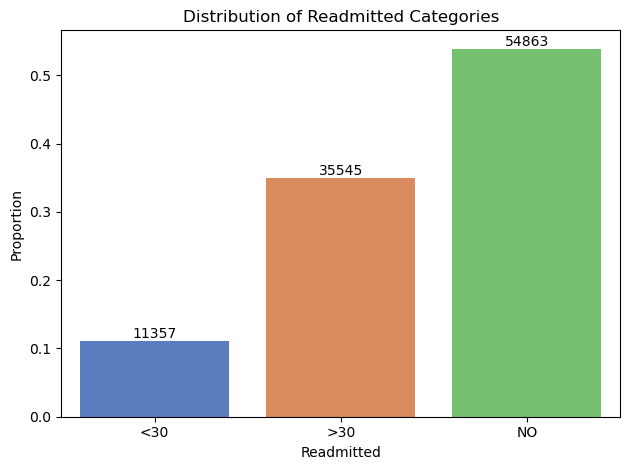
\includegraphics[width=0.80\textwidth]{plt_targetProportions.png}
	\caption{Barplots of proportions of encounters in each \texttt{readmitted} class. The classes are imbalanced with more than half in the not readmitted class and the fewest in the early readmission class. Counts for each class are shown on top of the bars.}
	\label{fig:target_barplot}
\end{figure}

\subsection{Missing Data Handling and Preprocessing}

The lab testing variables \texttt{max\_glu\_serum} and \texttt{A1Cresult} each had four categorical levels in the raw dataset, including a category \texttt{none}, indicating that the test wasn't conducted. To avoid confusion, I recoded this to \texttt{untested}. I could've split each of these into two features---one binary (tested or not) and one ordinal for results (normal, elevated or high). Instead, I opted to one-hot encode the four categorical levels as is. 

Several variables had missing values recorded as question marks in the raw dataset. These were race, medical specialty, payer code, weight, and the three diagnosis code variables.

For race, missing values (2.2\% of observations) showed some small trends: patients from the emergency room or with missing payer codes were less likely to have missing race, while those with urgent admissions were more likely. Patients might not have disclosed their race, or some sources may have recorded hard to categorize races as question marks. Rather than imputing with the mode (Caucasian) or trying to model the missingness, I created an \texttt{Unreported} category to preserve this information.

Medical specialty had the highest rate of missing values, with nearly 50\% of records missing. The next largest category was internal medicine. Without clear patterns in the missingness, I created an \texttt{Unknown} category rather than imputing values.

About 40,000 records were missing payer code, including every encounter ID below 72091308 (indexes 0-20445). The remaining missing values appeared random. Since the missing category was the most frequent, I treated it as its own \texttt{Unknown} category rather than imputing another value.

The admission and discharge variables (\texttt{admission\_type\_id}, \texttt{admission\_source\_id}, and \texttt{discharge\_disposition\_id}) were composed of integer-coded categorical levels. They each contained two or more categories that could represent missing values (null, not available, not mapped). In admission type, 5.2\% were null, and another $\sim$5\% were not available or not mapped. All but 4 of the null values also had missing payer codes, suggesting they were missing at random. I remapped the admission type integer codes to the corresponding category and retained all the missing categories. 

For admission source, there were $\sim$7000 null or not mapped values. All 161 not mapped values were in the first 6000 observations with one exception. Otherwise, I didn't detect a pattern. These could be grouped or imputed with the mode (emergency room). I opted to leave them as is and converted the datatype to avoid implying order.

Fewer than 5000 values in discharge disposition could be considered missing, mostly null and the rest not mapped. They appeared randomly scattered. I kept them as is and converted them to categorical. 

96.9\% of observations were missing weight. It didn't make sense to impute nearly the entire column, so I dropped it.

I dropped the examide and citoglipton variables because of zero variance. All the values were identical and provided no information to separate target classes. I also dropped the ID variables, \texttt{encounter\_id} and \texttt{patient\_nbr}.

\subsection{Encoding and Scaling}

Fewer than 2\% of observations had missing diagnosis codes. Since it's reasonable that not every patient would have multiple diagnosis codes, I didn't impute missing values. One observation had no listed diagnosis codes but a \texttt{number\_diagnosis} value of 5, which might have been a recording error.

I used a multi-column count encoding. Each observation got a vector of diagnosis code counts (ranging from one to three, about 98\% of observations had three). I dropped the observation with no diagnosis codes to avoid missing values rather than choosing to impute the mode for diagnosis code 1. I created a column for each unique diagnosis code and recorded the count of each code per encounter. Each diagnosis variable had 717-790 unique codes, but there was substantial overlap, leaving $\sim$900 unique codes. About 6\% of patients had duplicate codes (or after count encoding, a count of more that one for a code).

I one-hotencoded the remaining categorical variables, dropping the first category to prevent multicollinearity. For k levels, this created k-1 dummy variables, with the dropped category becoming the reference level. I considered converting age to a numeric variable, and using the middle of the range as the value for each observation. I decided against this, because I didn't want to assume a linear relationship between age and readmission risk. Another option would have been to give age a numeric value based on the ordinal scale, but again, I decided to treat it as categorical and sacrifice the ordinal information. 

Because many of the numerical variables were not normally distributed and had high outliers, I opted for a robust scaler to scale the data.

\section{Modeling}

A logistic regression model was chosen for its high interpretability and computational efficiency. 

Several steps went into my search for the best model parameters. I started by comparing two solvers, \texttt{saga} (Stochastic Average Gradient Augmented) and \texttt{lbfgs} (Limited-memory BFGS), at several values of the regularization parameter \texttt{C}. I used a grid search and stratified shuffling of the target variable with 5-fold cross-validation, optimizing for the mean out-of-fold weighted F1 score. I chose this metric because I wanted to prioritize identifying patients at risk of readmission, while also minimizing incorrect readmission predictions.

F1 score balances recall (also called sensitivity), the proportion of correctly predicted positives out of all actual positives, and precision (or positive predictive value), the proportion of correctly predicted positives out of all predicted positives. This is important because it helps ensure that at risk patients receive appropriate care, while avoiding unnecessary interventions for those who are not truely at risk. I chose weighted F1 score because of the imbalance in the target classes.

I expected \texttt{saga} to perform well because the dataset contains over 1000 features (after encoding), 100,000+ records, and many sparse features from high-cardinality categorical variables. By using stochastic gradient descent, it is designed for use with large, sparse datasets. However, it was significantly slower, over 12 minutes for a single fit compared to 38 seconds for \texttt{lbfgs} at \texttt{C=1} with only 0.04\% improvement in weighted F1. That made me realize that, despite its size, this dataset is still small enough to fit in memory and might be better suited to solvers that batch process like \texttt{lbfgs}.

Next, I compared \texttt{lbfgs} with \texttt{newton-cg} (Newton's method using the Conjugate Gradient algorithm) expanding the range of \texttt{C} values up to 10 and 100. Although \texttt{newton-cg} at \texttt{C=100} resulted in the the highest weighted F1 score, the improvement over \texttt{lbfgs} was minimal at just 0.04\%. I ultimately chose \texttt{lbfgs} for its robustness. Rather than computing a Hessian matrix (a matrix of second derivatives for precise optimization) directly, it approximates one. This can make it less sensitive to poor initial conditions and local minima. 

I ultimately chose the Scikit-Learn's logistic regression model's default parameters, \texttt{solver=lbfgs} and \texttt{C=1.0}. A weaker regularization parameter, \texttt{C=10} resulted in a minimal increase in weighted F1, 0.02\% but increased computation time by nearly double.

Rather than using \texttt{class\_weight='balanced'}, which sets the weight of each class inversely proportional to its frequency in the data, I also tuned \texttt{class\_weight} to optimize the weighted F1 score. I selected weights of 2 for the \texttt{\textless 30} class, 1.5 for the \texttt{\textgreater 30} class and 1 for the \texttt{NO} class, increasing the importance of the two less frequent classes. This weighting was not as extreme as given by the balanced class weight paramenter, which is based on the class proportions.

I also optimized the classification threshold for the \texttt{\textless 30} class, choosing a threshold which optimized F1 score on 5-fold cross validated predictions. This prioritized trade-offs in performance for detecting early readmissions.

\section{Results}

\subsection{Model Performance and Threshold Tuning}

I chose to examine Precision-Recall (PR) curves over ROC curves because I prioritized these two metrics in this analysis. Recall measures the proportion of actual positive cases that were correctly identified, while precision measures the proportion of predicted positive cases that were actually positive. As recall increases and more true positives are correctly classified, typically there are also more false positives, decreasing precision. These show the trade-offs between correctly identifying positive cases (recall) and avoiding false positives (precision). In this scenario, I wanted to maximize both metrics, particularly for the early readmission class.

In Figure 2, PR curves for each readmission class (Top: early readmission, Middle: later readmission, Bottom: not readmitted) show the trade-off between these two metrics. The threshold which optimizes F1 score for each class is shown in red, and the threshold selected for optimizing for the \texttt{\textless 30} class is marked by the yellow \texttt{X} in the middle and bottom plots.

ROC curves can be misleading in imbalanced datasets because they plot true positive rate (sensitivity) against false positive rate (1-specificity). If a positive class is rare, then a model can still achieve high scores in both by predicting mostly negative cases. PR curves help show how well a model performs on the minority class.

The weighted one-versus-rest area under the ROC curve (AUC-ROC) was 0.6798 (Table 3), with individual class AUC-ROC values 
of 0.67 for early, 0.66 for later, and 0.70 for no readmission (Table 4). To find the weighted AUC-ROC, these 
individual values are weighted by the proportion of each class in the dataset (11.1\%, 34.9\%, and 53.9\% respectively). This is a 
threshold-independent metric of model performance that accounts for the class imbalance.

\begin{figure}[h]
    \centering
    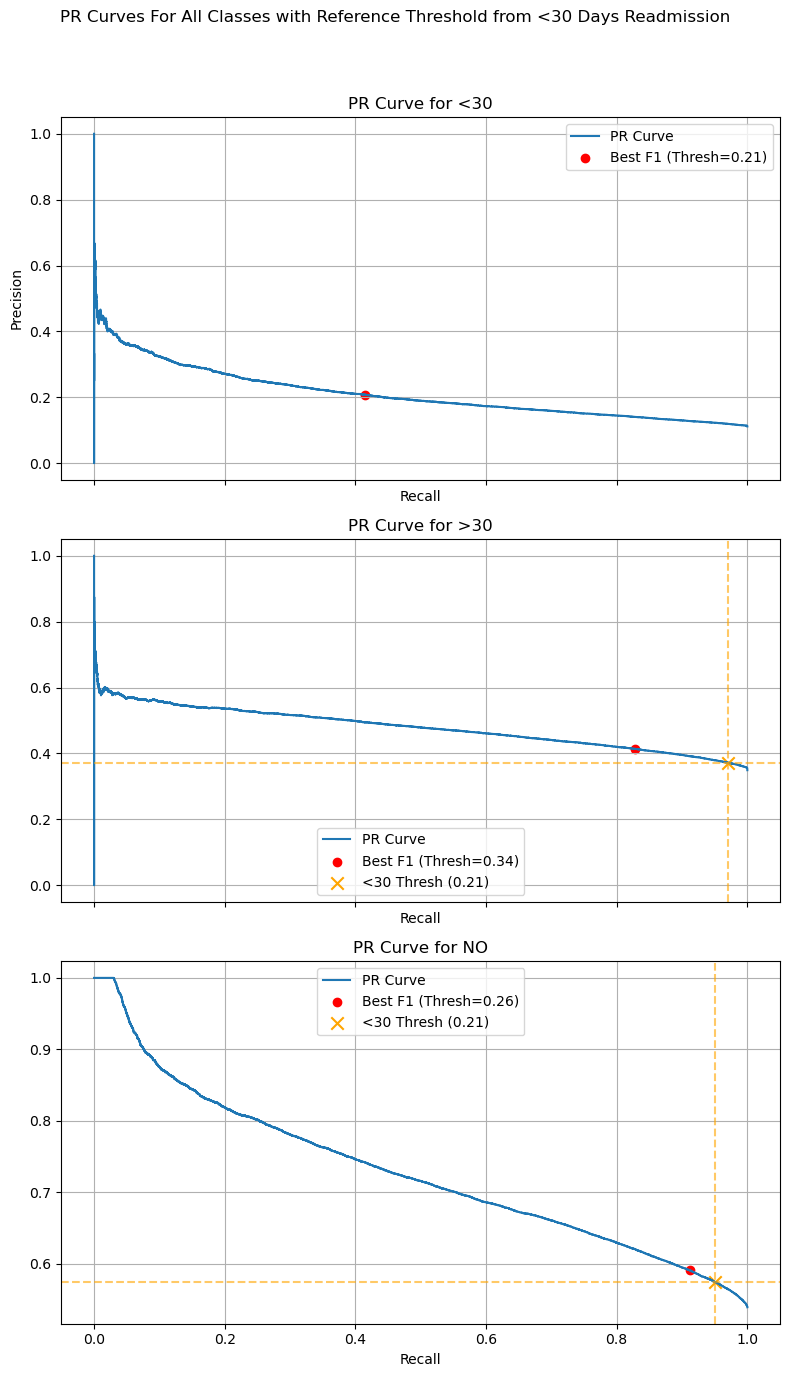
\includegraphics[width=0.90\textwidth]{plt_prCurves_vert.png}
    \caption{Precision-Recall curves for each class. The threshold which achieves the highest F1 score for each class is marked by the red circle and the chosen threshold is shown by the yellow \texttt{X}.}
    \label{fig:prCurves}
\end{figure}

\FloatBarrier
Table 3 contains the overall metrics from the cross-validated model with the optimized \texttt{\textless 30} threshold.

\begin{table}[h!]
    \centering
    \captionof{table}{Overall Cross-Validated Out-Of-Fold Metrics} 
    \begin{tabular}{|l|c|c|}
    \hline
    \textbf{Metric} & \textbf{Mean} & \textbf{Standard Deviation} \\ \hline
    Weighted F1-score & 0.5529 & 0.0039 \\ \hline
    Weighted Recall & 0.5145 & 0.0058 \\ \hline
    Weighted Precision & 0.5518 & 0.0033 \\ \hline
    Weighted AUC & 0.6798 & 0.0036 \\ \hline
    Accuracy & 0.5145 & 0.0040 \\ \hline
    \end{tabular}
    \label{table:overall_metrics}
\end{table}

\FloatBarrier
Table 4 contains results from the classification report after optimizing the \texttt{\textless 30} threshold for F1 score.

\begin{table}[h!]
    \centering
    \captionof{table}{Metrics by Readmission Class} 
    \begin{tabular}{|l|c|c|c|}
    \hline
    \textbf{Metric} & \textbf{\textless 30} & \textbf{\textgreater 30} & \textbf{NO}\\ \hline
    F1-score & 0.2771 & 0.4271 & 0.6373 \\ \hline
    Recall & 0.4154 & 0.4014 & 0.5963 \\ \hline
    Precision & 0.2079 & 0.4562 & 0.6844 \\ \hline
    AUC & 0.6681 & 0.6562 & 0.6975 \\ \hline
    \end{tabular}
    \label{table:class_metrics}
\end{table}

The confusion matrices, in Figure 3, help demonstrate the trade-offs in optimizing the classification threshold for the \texttt{\textless 30} class. Using the default threshold (upper matrix), the \texttt{argmax}, only 1016 \texttt{\textless 30} patients were correctly classified. Yet $\sim$21,000 \texttt{\textgreater 30} and $\sim$35,000 \texttt{NO} classifications were correct. Lowering the threshold to 0.21 to optimize for correct predictions in the early readmission class (lower matrix) increased the number of correct predictions in that class to 4718 but also drastically increased the number of incorrect early readmission predictions from roughly 2000 to 18,000. This also reduced the correct \texttt{\textgreater 30} and \texttt{NO}  predictions to $\sim$14,000 and $\sim$32,000, respectively. 
This will likely increase the cost of care for many patients, but with the hope of improving outcomes for those at risk.

\begin{figure}[h]
    \centering
    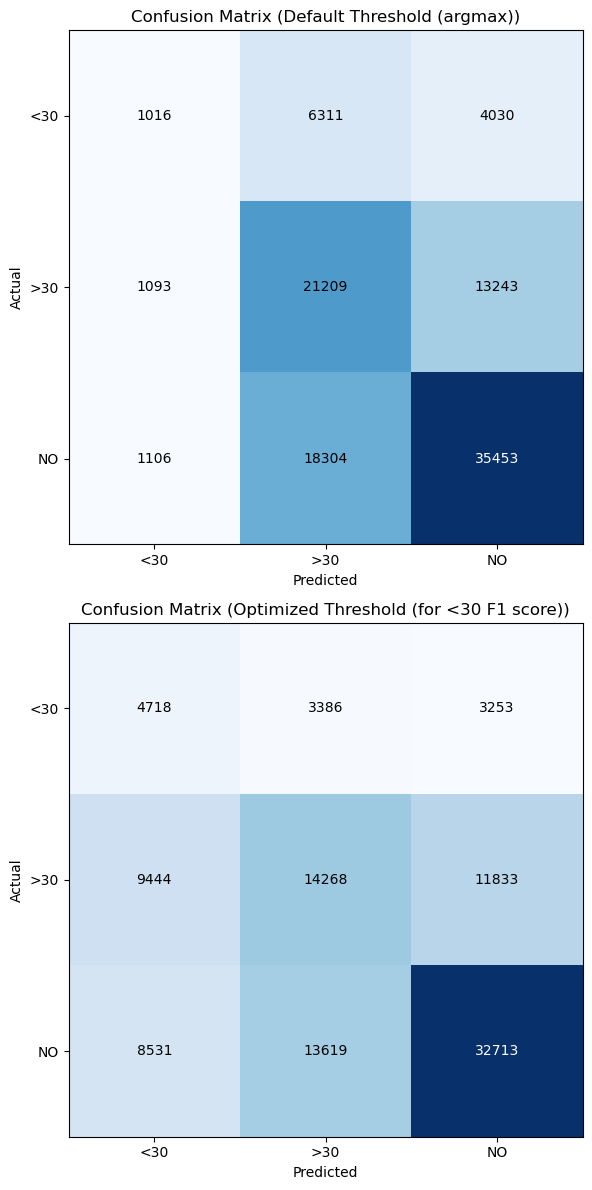
\includegraphics[width=0.75\textwidth]{plt_cm_optimized_vert.png}
    \caption{Confusion matrixes for the tuned model with both the default (\texttt{argmax}) (Top) and optimized \texttt{\textless 30} (Bottom) thresholds.}
    \label{fig:confusionMatrices}
\end{figure}

\subsection{Class-Specific Metrics}

Optimizing the \texttt{\textless 30} threshold increased the recall for the early readmission class from 9\% to 42\% and its F1 score from 14\% to 28\% but reduced its precision from 32\% to 21\%, as shown in Table 4. The improved classification in early readmissions lowered recall in the other classes and F1 score in the later readmissions. It also lowered the overall accuracy from 57\% to 51\% (Table 3). 

This trade-off suggests that prioritizing detection of patients with higher risk of early readmission comes primarily at a cost of detecting later readmissions. 

\subsection{Feature Importance}

Figure 4 displays bar plots of the five most important features and their coefficients from each readmission class (Top: early readmission, Middle: later readmission, Bottom: not readmitted). The features and their descriptions are listed in Table \ref{table:important_variables}. Three larger variable categories stand out: discharge disposition, admission type and diagnosis. The most important feature in determining all the classes is discharge disposition 11, the code for expired. Of course, if a patient died, they were not readmitted. Unfortunately, that information is unlikely to help prevent future readmissions. Diagnosis code 14, to a hospice/medical facility, is not a strong predictor of early readmission, but it does have a negative association with later readmissions and a positive one with not readmitted. Additionally, admission through a trauma center is positively associated with not being readmitted. 

The rest of the important variables are specific diagnoses. Two diagnoses are important predictors of early versus late readmissions. Both tick-borne rickettsioses (82) and disorders of carbohydrate transport and metabolism (271) are positively associated with early readmission and negatively associated with late readmission. Other strong positive predictors of early readmission are rheumatic fever with heart involvement and respiratory conditions due to chemical fumes and vapors. A strong predictor of late readmission is a diagnosis of cataract. One can speculate, but this may be confounded by age. Foot fracture and jaw disease were somewhat surprisingly negatively associated with not being readmitted. 

\begin{figure}[h]
    \centering
    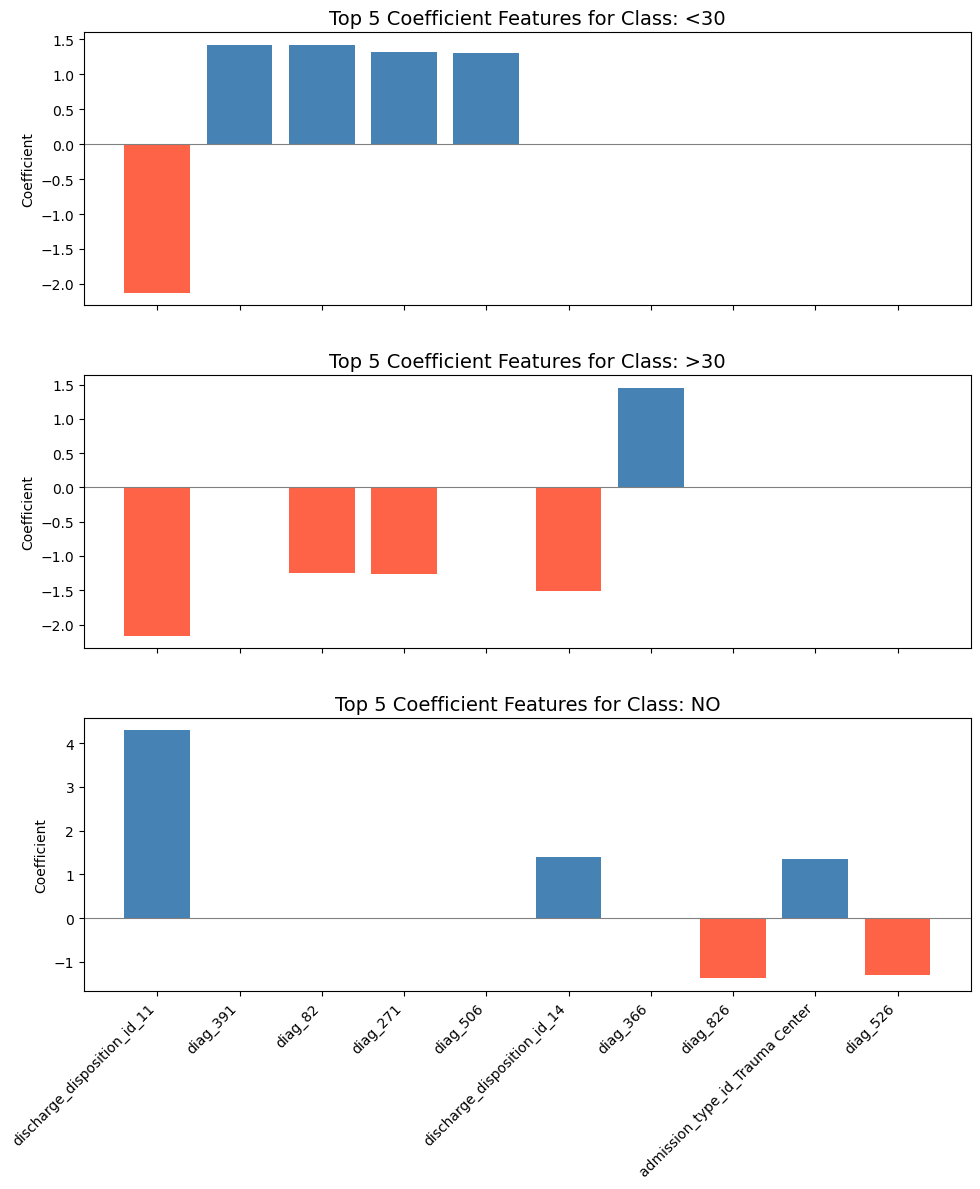
\includegraphics[width=1.0\textwidth]{plt_top5vars_perClass.png}
    \caption{Top five most important features for each class.}
    \label{fig:Top5Vars_perClass}
\end{figure}

\FloatBarrier
Table 5 contains the five most important features for each of the readmission classes and their description. Some classes share important features.

\begin{table}[h!]
    \centering
    \captionof{table}{Most Important Features of all Readmission Classes} 
    \begin{tabular}{|l|p{9cm}|}
    \hline
    \textbf{Variable} & \textbf{Description} \\ \hline \hline
    discharge\_disposition\_id\_11 & expired \\ \hline
    discharge\_disposition\_id\_14 & hospice/medical facility \\ \hline
    admission\_type\_id\_Trauma Center & admission via Trauma Center \\ \hline
    diag\_391 & Rheumatic fever with heart involvement \\ \hline
    diag\_82 & Tick-borne rickettsioses \\ \hline
    diag\_271 & Disorders of carbohydrate transport and metabolism \\ \hline
    diag\_506 & Respiratory conditions due to chemical fumes and vapors \\ \hline
    diag\_366 & Cataract \\ \hline
    diag\_826 & Fracture of one or more phalanges of foot \\ \hline
    diag\_526 & Diseases of the jaws \\ \hline
    \end{tabular}
    \label{table:important_variables}
\end{table}

\section{Conclusion}

Optimizing the classification threshold for the early readmission (\texttt{\textless30}) class resulted in many more true positives but also increased false positives for that class. However, it drastically reduced false negatives (from the \texttt{NO}, not readmitted class). This improvement in sensitivity (recall) came at a cost of reduced accuracy for both the later readmission (\texttt{\textgreater 30}) and the not readmitted (\texttt{NO}) classes.

Based on recall scores, the model correctly identified 41.5\% of patients readmitted within 30 days, 40.1\% of those readmitted after 30 days, and 59.6\% of those not readmitted.

Several diagnoses are associated with early readmission: tick-borne disease, carbohydrate metabolic disorder, rheumatic fever involving the heart and respiratory conditions due to fumes. 

An important consideration from the feature importance results is whether demographic variables like race, gender, and age should be included in a similar model going forward. There are pros and cons to consider. There may be a slight predictive advantage in including these. Perhaps certain subgroups are at greater or lesser risk and knowing that, the best treatment options could be prioritized. This also introduces the possibility of bias. One option would be to code these variables and let only certain individuals have access to the true categories. Of course, these variables may be confounded by others like payer code or comorbidities. Examining multicollinearity may be helpful. One option would be to exclude these variables from the final model, but retain the information for monitoring associations with readmission or correlations with other variables in future models.

\end{document}
